%!TEX TS-program = xelatex
%!TEX encoding = UTF-8 Unicode

\documentclass[12pt]{article}
\usepackage{geometry}                % See geometry.pdf to learn the layout options. There are lots.
\geometry{a4paper,top=2cm}
\usepackage[parfill]{parskip}    % Activate to begin paragraphs with an empty line rather than an indent
\usepackage{graphicx}
\usepackage{amsmath}
\usepackage{amssymb}
\usepackage{mathtools}
\usepackage{physics}
\newcommand{\be}{\begin{equation}}
\newcommand{\ee}{\end{equation}}
\usepackage[thicklines]{cancel}
\usepackage[colorlinks=true,citecolor=blue,linkcolor=blue,urlcolor=blue]{hyperref}
\usepackage{booktabs}
\usepackage{csquotes}
\usepackage{qcircuit}
\usepackage{circledsteps}
\usepackage{nicefrac}
\usepackage{fontspec,xltxtra,xunicode}
\usepackage{xcolor}
\usepackage{simplewick}
\defaultfontfeatures{Mapping=tex-text}

\newcommand{\polv}{\ensuremath{\updownarrow}}
\newcommand{\polh}{\ensuremath{\leftrightarrow}}
\newcommand{\poldr}{\rotatebox[origin=c]{45}{\ensuremath{\leftrightarrow}}}
\newcommand{\poldl}{\rotatebox[origin=c]{-45}{\ensuremath{\leftrightarrow}}}
\newcommand{\bigzero}{\mbox{\normalfont\Large\bfseries 0}}
\newcommand{\vecrp}{\ensuremath{\vec{r}^{\,\prime}}}
\newcommand{\vecnr}{\ensuremath{\vec{\nabla}_{\!r}}}

\title{Advanced Quantum Mechanics\\Class 10}
%\author{The Author}
\date{September 06, 2022}                                           % Activate to display a given date or no date

\setcounter{section}{5}
\setcounter{subsection}{8}
\setcounter{equation}{104}

\begin{document}
\maketitle

%%% 1 OK
\subsection{Interference and entangled states}

Consider decay of an unstable particle (at
``rest") into two other stable particles $a$ and $b$, in which
%%% 2 OK
one of them is made to pass through a Young's
slit apparatus:
\be
\vec{p}_1 + \vec{p}_2 = 0
\ee

\begin{minipage}{0.5\textwidth}
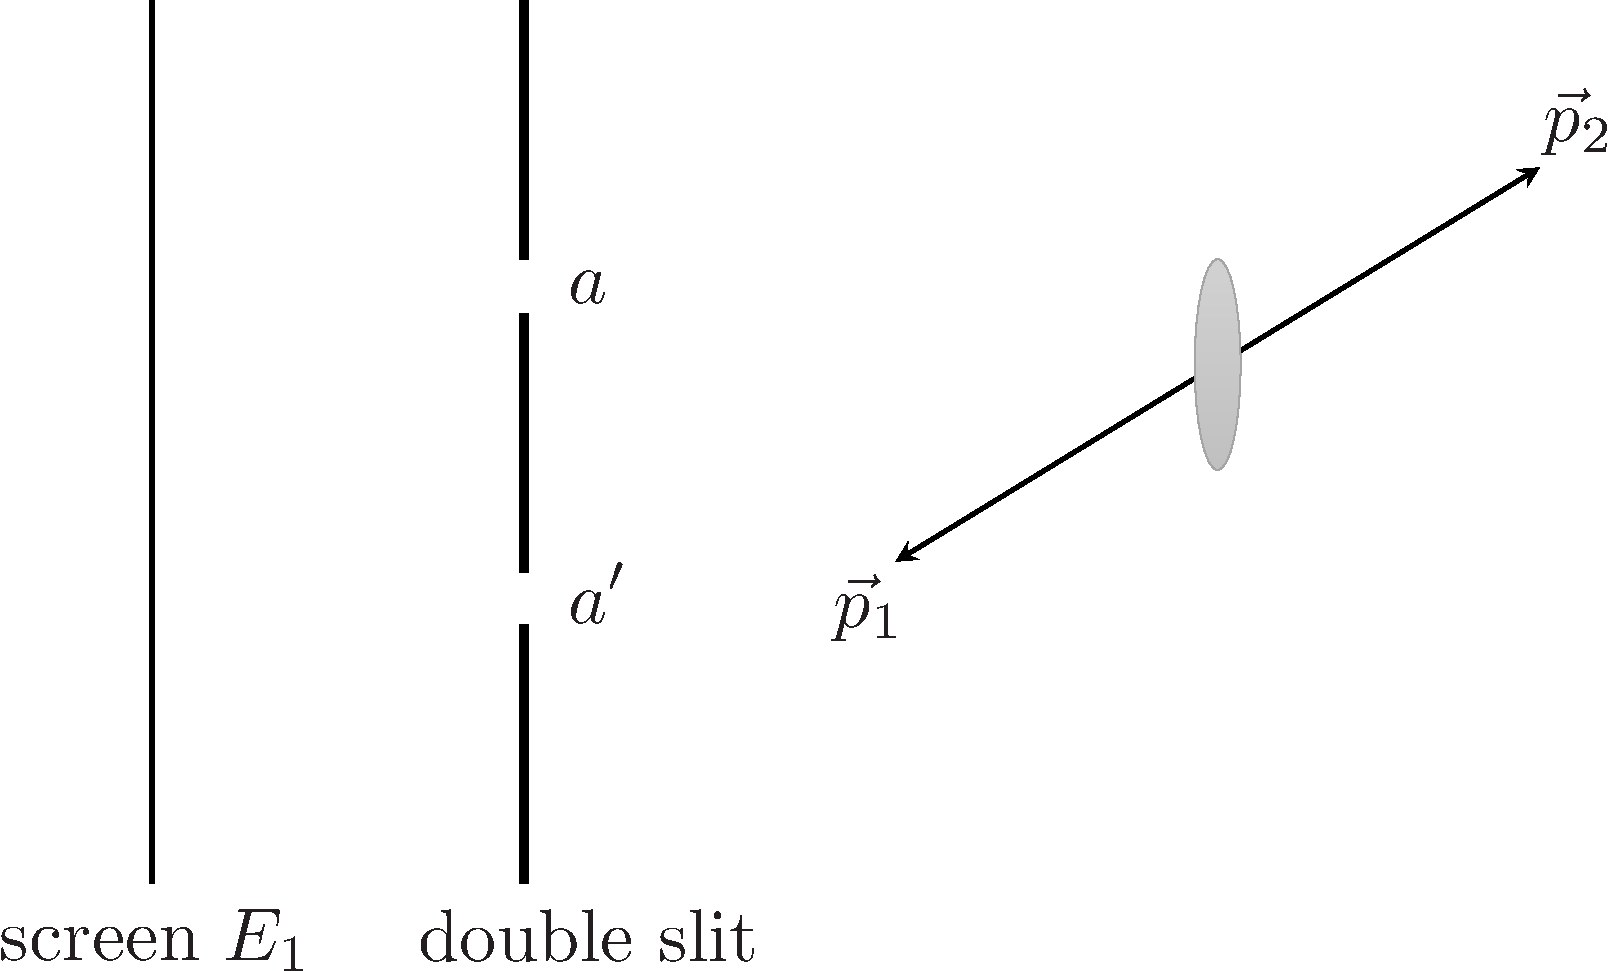
\includegraphics[width=\textwidth]{Figures/DoubleSlitEntangled.pdf}
\end{minipage}%
\begin{minipage}{0.5\textwidth}
\[
\left\{
\begin{aligned}
|a\rangle: & \text { state when particle } \\ 
& \text { passes slit $a$ when } \\ 
& \text { $a^{\prime}$ is closed } \\
|a^{\prime}\rangle:
& \text { reverse situation of } \\
& \text { the above } 
\end{aligned}
\right.
\]
\end{minipage}

Suppose initial state is an entangled state:
\be
\ket{\psi} = \frac{1}{\sqrt{2}}
\left(
\ket{a}\otimes\ket{b} + \ket{a^\prime}\otimes\ket{b^\prime}
\right)
\ee

\emph{Question:} will there be an interference pattern
on screen \(E_{1}\)?

\emph{Answer:} No. Why not? Because, even if particle 1
is not disturbed, it is \emph{possible in principle}
to know its trajectory when particle 2 is
detected with a suitable apparatus.
\begin{center}
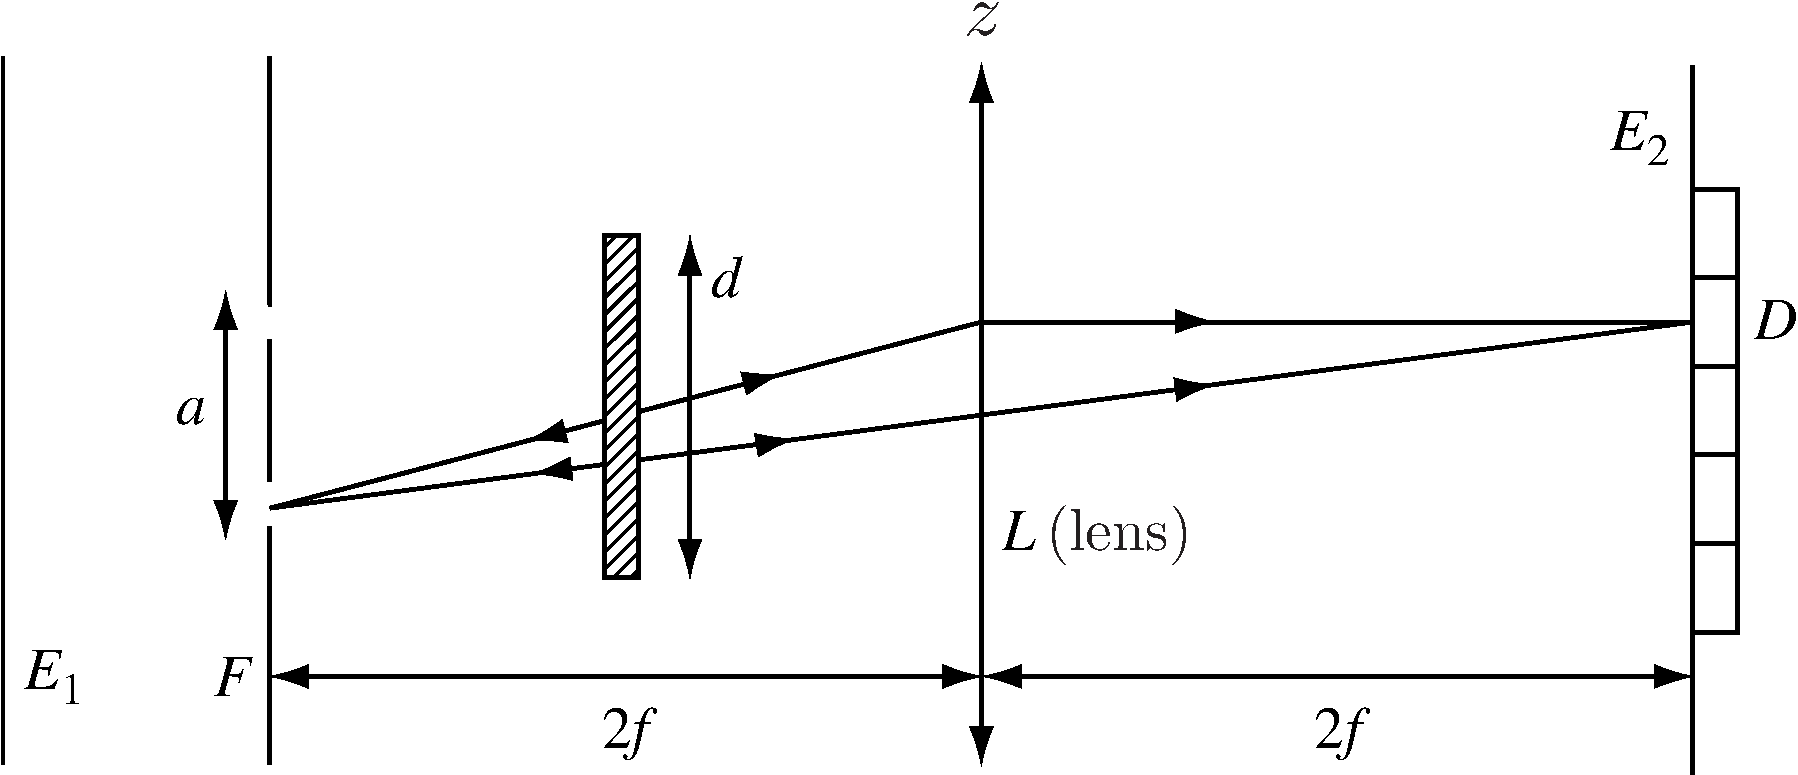
\includegraphics[width=0.8\textwidth]{Figures/InterferenceEntangled1.pdf}
\end{center}

Detection of particle 2
without disturbing 1
allows us to determine
trajectory of 1 (within
uncertainty in the vertical
component of momentum: $\delta p_z d \sim \hbar$).

%%% 3 OK
Therefore: detection of particle 2 will give information
on which slit particle 1 has passed through.
\begin{itemize}
\item no interference pattern
\item no need for the lens and detector \(D\), only
the fact that in principle one can do
such an experiment
\item it is the existence of the second (entangled,
due to momentum conservation \(\vec{p}_{1}=-\vec{p}_{2}\) ) that
is crucial
\end{itemize}
One can obtain an interference pattern by measuring
the direction of the momentum of particle 2:
\begin{center}
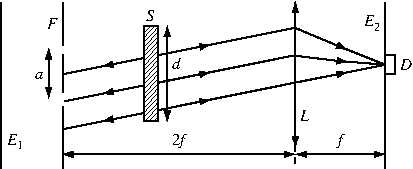
\includegraphics[width=0.8\textwidth]{Figures/InterferenceEntangled2.pdf}
\end{center}

One can determine the
direction of the momentum
of 2 before the lens $\to$
\emph{therefore also of 1}.
But then no trace of position of 1, and
interference pattern is back, because we
have forced particle 2 in some direction,
the focal point. Recall: the particles
were entangled in momentum.

%%% 04 OK
\subsection{GHZ states: three-particle entanglement}

GHZ: Greenberger - Horne - Zeilinger (1989), \emph{Going Beyond Bell's Theorem}, \url{https://arxiv.org/abs/0712.0921}
\be
\ket{\psi} = \frac{1}{\sqrt{2}}
\left(\ket{+++} - \ket{---}\right)
\ee
They are emitted in a plane, in a $0$--$120^\circ$--$240^\circ$ configuration 
(see figure in the next page).
\begin{center}
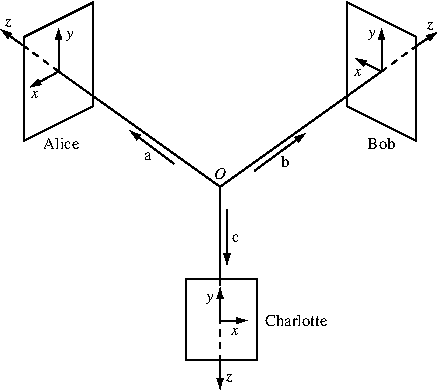
\includegraphics[width=0.8\textwidth]{Figures/GHZExperiment.pdf}
\end{center}

Alice (a), Bob (b), Charlotte (c) measure the spin component
in the direction perpendicular to the
direction of propagation of each particle.
Each particle
has its own $z$ axis, but all
have same $x$ and $y$ axes.

Consider the three operators:
\be
\begin{aligned}
\Sigma_{a}=\sigma_{a x} \sigma_{b y} \sigma_{c y}\\
\Sigma_{b}=\sigma_{a y} \sigma_{b x} \sigma_{c y}\\
\Sigma_{c}=\sigma_{a y} \sigma_{b y} \sigma_{c x}\\
\end{aligned}
\ee
$\to$ note position of $\sigma_x$.
\(\sigma_{i}\) acts in the spin space of particle \(i: i=a, b, c\)
Index \(i\) in \(\Sigma_{i}\) : position of \(\sigma_{x}\) in the product abc.

%%% 05 OK

\emph{Exercise:}
\be
\left[\Sigma_{i} \Sigma_{j}\right]=0,
\quad
\Sigma_{i}^2 = \mathbf{1}
\ee
so the $\Sigma_{i}$ have simultaneous reality, and their eigenvalues are $\pm1$.
%
\be
\Sigma_{a}|\psi\rangle=|\psi\rangle \quad \Sigma_{b}|\psi\rangle=|\psi\rangle \quad \Sigma_{c}|\psi\rangle=|\psi\rangle
\ee
%
\be
\Sigma \equiv \sigma_{a x} \sigma_{b x} \sigma_{c x}=-\Sigma_{a} \Sigma_{b} \Sigma_{c}
\ee
which means:
\be
\Sigma|\psi\rangle=-|\psi\rangle
\label{eq:g112}
\ee
\be
[\Sigma, \Sigma_i]=0
\ee
All four combinations can be measured simultaneously
For axes in direction \(x, y, y\), combination \(\sigma_{x} \sigma_{y} \sigma_{y}\)
is measured. When measuring on \(|\psi\rangle \rightarrow\) result is \(+1\).
Same result when using axes \(y, x, y\) and \(y, y, x\).
Moreover, when the configuration of the axes is
\(x, x, x\), result of measurement is \(-1\), due to Eq.~\eqref{eq:g112}.

To compare with predictions of local realism, let us
denote \(A_x\) measurement of \(\sigma_{x}\) by Alice, \(B_{x}\) measurement 
of \(\sigma_{x}\) by Bob, \ldots\ \(C_{y}\) measurement of \(\sigma_{y}\)
by Charlotte. We have that
\be
A_{x}=\pm 1, B_{x}=\pm 1, \ldots, C_{y}=\pm 1
\ee

%%% 06 OK

According to \emph{quantum mechanics}:
\be
A_{x} B_{y} C_{y}=+1, \quad A_{y} B_{x} C_{y}=+1, \quad A_{y} B_{y} C_{x}=+1
\label{eq:g115}
\ee
and, due to Eq.~\eqref{eq:g112}.
\be
A_{x} B_{x} C_{x}=-1
\label{eq:g116}
\ee
\emph{Important here:} the value of \(A_x\), for example is
\emph{contextual:} it depends on the other
spins with which \(\sigma_{x}\) is measured
$\rightarrow$
\(\sigma_{x}\) is incompatible with \(\sigma_{y}\), therefore
\(A_{x}\) in \(A_{x} B_{y} C_{y}\) \emph{is not} the same as
in \(A_{x} B_{x} C_{x}\) : in the first case, \(\sigma_{x}\) is
measured together with \(\sigma_{y}\) while in
the second it is measured with \(\sigma_{x}\).

Now, according to \emph{local realism}, there is no
such a thing as incompatible properties, \textit{i.e.}
\(A_{x}\) in \(A_{x} B_{y} C_{y}\) is the same as in \(A_{x} B_{x} C_{y}\).
\emph{Consequence:} inserting $A_y^2 = B_y^2 = C_y^2 = 1$
in the right places, and moving them around
(there are no ``incompatible operators'' in local realism, so everything commutes):
\be
A_{x} B_{x} C_{x}=A_{x} B_{y} C_{y}\cdot A_{y} B_{x} C_{y}\cdot A_{y} B_{y} C_{x}=+1
\ee
%%% 07 OK
Therefore, local realism would imply that Eq.~\ref{eq:g115}
is incompatible with Eq.~\ref{eq:g116} $\rightarrow$ quantum mechanics
leads to contradictory results! \emph{NO}, of course, the
error is supposing that \(A_{x}\) in \(A_{x} B_{x} C_{x}\) is the
same as in \(A_{x} B_{y} C_{y}\): they are not, \(A_{x}\) is contextual,
as discussed above. Remember,
it is not possible to measure simultaneously 
\(A_{x}, A_{y}, B_{x}, B_{y}, C_{x}, C_{y}\), they are
eigenvalues of operators that do not
all commute with each other.

\subsection{Measurement and decoherence}

Copenhagen interpretation of measurement in QM
\begin{itemize}
\item Apparatus is classical, operates according to
macroscopic laws.
\item It is not meaningful to regard a quantum
particle as possessing \emph{any} intrinsic property,
independent of the measuring apparatus used
to measure it $\rightarrow$ property is revealed only
when measured, before the measurement the
particle does not hove in general a well defined
property (collapse of the wave function).
\end{itemize}

%%% 08 OK

For some, this is problematic: if one believes that
the fundamental laws of physics are quantum laws
$\rightarrow$ classical physics is only an approximation:
\begin{itemize}
\item measuring means interacting with the quantum
particle at the microscopic level;
\item how is then this microscopic in interaction,
governed by quantum evolution (unitary), is
amplified so that a macroscopic signal
(\emph{e.g.} movement of a needle in a measuring
device) is produced?
\end{itemize}
This is ``explained'' by the phenomenon of \emph{decoherence}.

Suppose \(\left|\varphi_{+}\right\rangle\) and \(\left|\varphi_{-}\right\rangle\) possible states of the system.
Interaction of the apparatus with the system \(\rightarrow\) entanglement
system + apparatus:
\[
\begin{aligned}
\left|\varphi_{+} \otimes \psi_{+}\right\rangle:\quad
&\text {observation of apparatus, }\left|\psi_{+}\right\rangle, \\ 
&\text {informs on }\left|\varphi_{+}\right\rangle \\ 
\left|\varphi_{-} \otimes \psi_{-}\right\rangle:\quad 
&\left|\psi_{-}\right\rangle \text { informs on }\left|\varphi_{-}\right\rangle
\end{aligned}
\]
But suppose that the system is in a superposition:
%%% 09 OK
\[
\lambda\left|\varphi_{+}\right\rangle+\mu\left|\varphi_{-}\right\rangle 
\xrightarrow[\text{with apparatus}]{\text{interaction}} 
\lambda\left|\varphi_{+} \otimes \psi_{+}\right\rangle+
\mu\left|\varphi_{-} \otimes \psi_{-}\right\rangle
\]
where the right hand of this relation points to
linear superposition of
macroscopic states if apparatus
is macroscopic.

At this point we make the analogy with the (in-)famous Schrödinger's cat:
\(\left|\psi_{+}\right\rangle\) cat is alive,
\(\left|\psi_{-}\right\rangle\) cat is dead.

\emph{Classical objects:} described by a classical
statistical ensemble, \emph{not} a
state vector, created by irreversible
interactions with an environment
with which they interact.

\emph{Decoherence:} off-diagonal
elements of the state
vector of a macroscopic
object decay at a rate
mach faster than the natural decay
rate of \textit{e.g.} the energy of the object.

Sketch of a real experiment:

\begin{center}
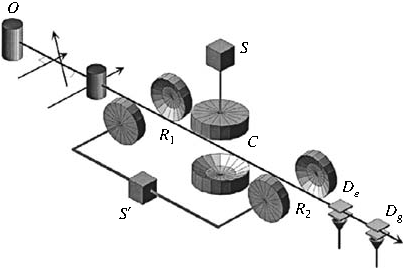
\includegraphics[width=\textwidth]{Figures/DecoherenceExperiment.pdf}
\end{center}

\emph{Oven O:} produces atoms
in ground $\ket{g}$ state
and in an excited $\ket{e}$
state.

\emph{Cavity C:} contains \mbox{e.m.} fields \(\simeq 10\) photons. When atoms
pass though C they change \(\Phi\) in the phase of
%%% 10 OK
the \mbox{e.m.} field (photons \emph{are not} absorbed by atoms,
off-resonance situation). The change in the phase
depends on the state of the atom.
Let \(|G\rangle\) be state of quantum state of field when
change in phase is \(+\Phi\) when atom in \(|g\rangle\) crossed
the cavity; likewise \(|E\rangle\) when change is \(-\Phi\) when
atom in \(|e\rangle\) crossed:
\be
\underbrace{|g G\rangle \text { and }|e E\rangle}_{\text {field + atom states}}
\ee

\emph{Microwave cavity $R_1$}: before entering $C$, atoms are
put in superposition states
according to:
\be
\begin{aligned}
|e\rangle \stackrel{R_{1}}{\longrightarrow}|a\rangle&=\frac{1}{\sqrt{2}}(|e\rangle+|g\rangle) \\ 
|g\rangle \stackrel{R_{1}}{\longrightarrow}|b\rangle&=\frac{1}{\sqrt{2}}(-|e\rangle+|g\rangle)
\end{aligned}
\label{eq:g119}
\ee
\emph{Suppose} that the oven $O$ has prepared atoms in
state $\ket{e}$. Then after passing through \(R_{1}\), the
interaction of the \mbox{e.m.} field and atom created the
entangled state
\be
|\Psi\rangle=\frac{1}{\sqrt{2}}\left(|e E\rangle+|g G\rangle\right)
\ee

%%% 11 OK

Now, after leaving \(C\), the atoms are made to pass through
a second microwave cavity, \(R_{2}\), which does what
\(R_{1}\) did: Eq.~\eqref{eq:g119}. That is, after leaving \(R_{2}\)
the state \(|\Psi\rangle\) of the atoms is modified to
\be
\begin{aligned}
|\Psi\rangle \stackrel{R_{2}}{\longrightarrow}\left|\Psi^{\prime}\right\rangle 
&=\frac{1}{\sqrt{2}}(|a E\rangle+|b G\rangle) \\ 
&=\frac{1}{\sqrt{2}}\left[\frac{1}{\sqrt{2}}(|e\rangle+|g\rangle)|E\rangle+\frac{1}{\sqrt{2}}(-|e\rangle+|g\rangle)|G\rangle\right] \\ 
&=\frac{1}{\sqrt{2}}\left[\frac{1}{\sqrt{2}}(|E\rangle-|G\rangle)|e\rangle+\frac{1}{\sqrt{2}}(|E\rangle+|G\rangle)|g\rangle\right] \end{aligned}
\ee

\emph{Recall:} \mbox{e.m.} field is the measuring
``device", the macroscopic object ( \(\approx\) 10 photons)
$\rightarrow$ not a terrible large number.
The measuring device (\mbox{e.m.} field)
was projected in a state of linear
superposition, \emph{after} the measurement
has occurred.

\emph{\(D_{e}\) and \(D_{g}\)}: ionization detectors, 
\(D_{e}\) for $\ket{e}$ and 
\(D_{g}\) for $\ket{g}$,
``measure'' the atoms \(\rightarrow\) they tell which
linear superposition the field is in (in $C$) $\rightarrow$ 
we set the macroscopic object (like the cat) 
in a linear superposition of states (live or dead)!
%%% 12 OK
\be
\begin{gathered}
\text {- when } D_{e} \text { is triggered } \rightarrow \frac{1}{\sqrt{2}}
\left(|E\rangle-|G\rangle\right) \\ 
\text {- when } D_{g} \text { is triggered } \rightarrow \frac{1}{\sqrt{2}}
\left(|E\rangle+|G\rangle\right)
\end{gathered}
\label{eq:g122}
\ee
One can learn about the state of the field in $C$
sending another atom (\textit{i.e.} send a mouse to test the cat) into
the cavity \(C\)$\rightarrow$ it can be shown experimentally that
the linear superpositions in Eq.~\eqref{eq:g122} are
very \emph{fragile} \(\rightarrow\) decoherence.

But what is decoherence? 
Suppose initially the field is in a pure state
\be
|\Phi\rangle=\lambda|E\rangle+\mu|G\rangle,\,|\lambda|^{2}+|\mu|^{2}=1
\ee
The corresponding state operator in the basis of $\{\ket{E},\ket{G}\}$ is
\be
\rho_{\text{in}}=\begin{pmatrix}|\lambda|^{2} & \lambda \mu^{*} \\ \lambda^{*} \mu & |\mu|^{2}\end{pmatrix}
\ee
and through decoherence
\be
\rho_{\text{fin}}=\begin{pmatrix}|\lambda|^{2} & 0 \\ 0 & |\mu|^{2}\end{pmatrix}
\ee
What causes this? Imperfections of cavity $C$, leaks
%%% 13 OK 
of photons due to imperfections in the mirrors that
keep the photons trapped in $C$ $\rightarrow$
off-diagonal terms contain information
on the relative phases \(\rightarrow\) tend to zero
very fast.

Evolution $\hat{\rho}_{\text {in}} \rightarrow \hat{\rho}_{\text {fin}}$ is nonunitary, 
\textit{i.e.} it is not governed by a Hamiltonian.

Interaction of the field with the environment leads
to a field + environment entangled state
$\rightarrow$ state operator if the field is then
\be
\hat{\rho}_{\text{field}}=\Tr_{\text{env}}\left(\hat{\rho}_{\text{field+env}}\right)
\ee
so the loss of information on the field to
the environment leads to an
increase in the entanglement entropy
of the field:
\be
S_{E}\left(\hat{\rho}_{\text{fin}}\right) \geqslant S_{E}\left(\hat{\rho}_{\text{in}}\right)
\ee

\end{document}